\documentclass{beamer}

\usepackage[utf8]{inputenc}
\usepackage[T1]{fontenc}
\usepackage[francais]{babel}

\usetheme{Darmstadt}
\usecolortheme{seahorse}
\setbeamertemplate{footline}[frame number]

\usepackage{graphicx}

\AtBeginSection[]{
    \begin{frame}
        \frametitle{Plan}
        \tableofcontents[currentsection,hideothersubsections]
    \end{frame} 
}

\titlegraphic{
    \begin{columns}
        \column{.1\textwidth}
        
\includegraphics[width=\textwidth]{img/imag.eps}
        \column{.4\textwidth}
        
\includegraphics[width=\textwidth]{img/topSolid.eps}
    \end{columns}
}

\title{Simulation de pliage dans un outillage progressif}
\author{Ariane LEFEBVRE \and Pablo COVES\\[.5cm] Master 2 MIA Image et CAO \and 2012-2013\\[.5cm] Tuteurs: Christophe PICARD \and Frédéric PONTAROLLO}
\date{}

\begin{document}
\maketitle

\section{Introduction}
\subsection{Missler Software}
\begin{frame}
    \begin{itemize}
        \item Première solution CFAO dans les années 80.
        \item Les services TopSolid:
            \begin{itemize}
                \item Générale: modélisation, assemblage...
                \item Outillage: moules, matrices...
                \item Tôlerie: Design, découpe et mise-en-forme.
            \end{itemize}
    \end{itemize}
\end{frame}
\subsection{Outillage progressif}
\begin{frame}
    \begin{columns}
        \column{.3\textwidth}
        \begin{itemize}
            \item Poinçon.
            \item Dévêtisseur.
            \item Tôle.
            \item Matrice.
        \end{itemize}
        \column{.7\textwidth}
        \begin{figure}
            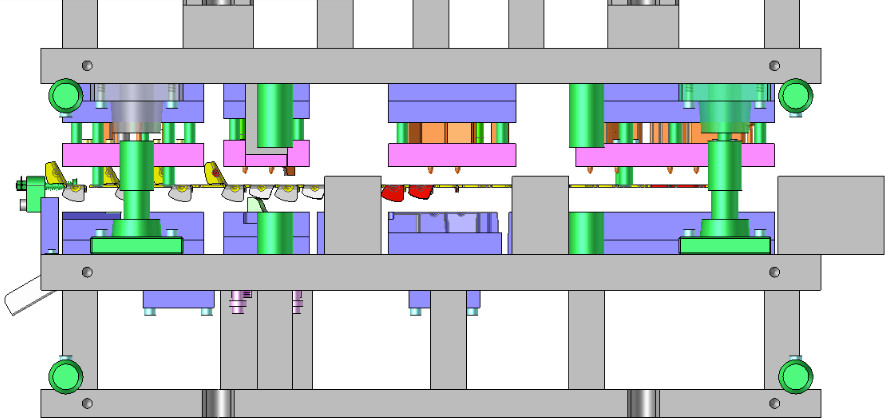
\includegraphics[width=\textwidth]{img/dieTool.jpg}
            \caption{Outillage progressif}
        \end{figure}
    \end{columns}
\end{frame}
\subsection{Opérations de base}
\begin{frame}
    \begin{itemize}
        \item Découpe:\\
            Ôte des morceaux des matériaux.
        \item Pliage:\\
            Modification de la forme de la tôle par formation d'angles.
        \item Poinçonnage:\\
            Forte pression provoquant une déformation.
    \end{itemize}
\end{frame}

\section{Contenu du projet}
\subsection{Projet du client}
\begin{frame}
    \frametitle{Spécifications}
    \begin{itemize}
        \item Application pour simuler en 2D une déformation réaliste.
        \item Retour élastique au retour du poinçon.
        \item Aire couverte par la tôle.
        \item Suivit d'un point en temps réel.
    \end{itemize}
\end{frame}
\begin{frame}
    \frametitle{Représentation 2D}
    \begin{columns}
        \column{.6\textwidth}
        \begin{itemize}
            \item \textbf{La matrice}: 
                Un polygone, fixe au cours du temps.
            \item \textbf{Le dévêtisseur}:
                Un polygone venant fixer la tôle à la matrice.
            \item \textbf{Le poinçon}:
                Un polygone en mouvement. Il vient frapper la tôle.
            \item \textbf{La tôle}:
                D'épaisseur fixe, elle est décrite par sa fibre neutre.
        \end{itemize}
        \column{0.4\textwidth}
        \begin{figure}
            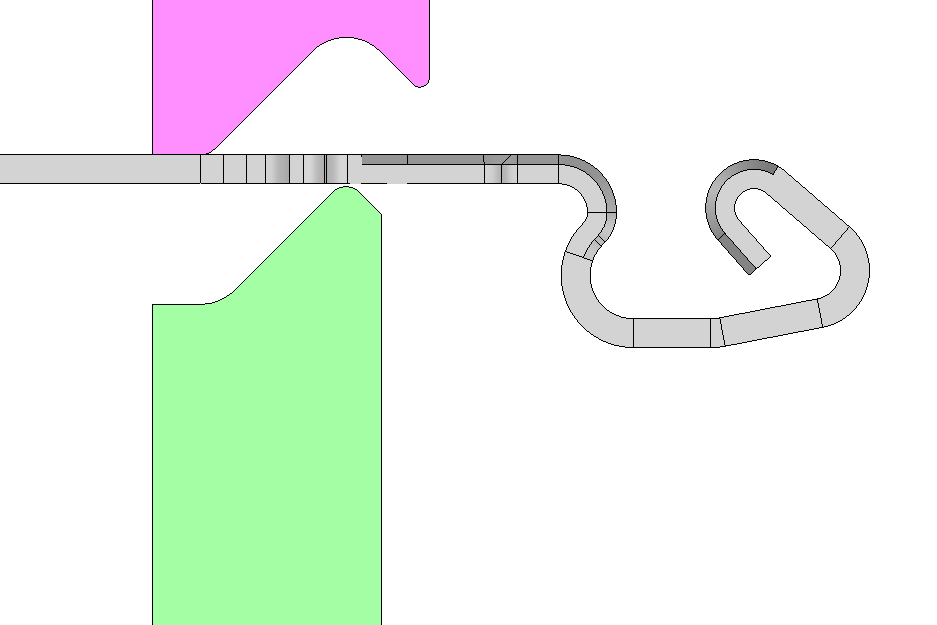
\includegraphics[width=\textwidth]{img/fibreNeutre.jpg}
            \caption{Représentation 2D}
        \end{figure}
    \end{columns}
\end{frame}
\subsection{Tâches à réaliser}
\subsubsection{Interface utilisateur}
\begin{frame}
    \frametitle{Interface utilisateur}
    Une fenêtre contenant:
    \begin{itemize}
        \item Des menus déroulant: choix des intéractions souris.
        \item Pas de temps entre chaque étapes.
        \item Temps totale de la simulation.
        \item Un lecteur pour la visualisation.
        \item Une zone de rendu OpenGL.
    \end{itemize}
\end{frame}
\subsubsection{Chargement d'une scène}
\begin{frame}
    \frametitle{Chargement d'une scène}
    Une scène est décrite par un fichier XML:
    \begin{itemize}
        \item Fourni par le client.
        \item Contient les caractéristiques du matériau.
        \item Contient les positions des éléments fixes.
        \item Contient les positions hautes et basses du poinçon.
    \end{itemize}
\end{frame}
\subsubsection{Moteur de déformations}
\begin{frame}
    \frametitle{Le moteur de déformation}
    \begin{figure}
        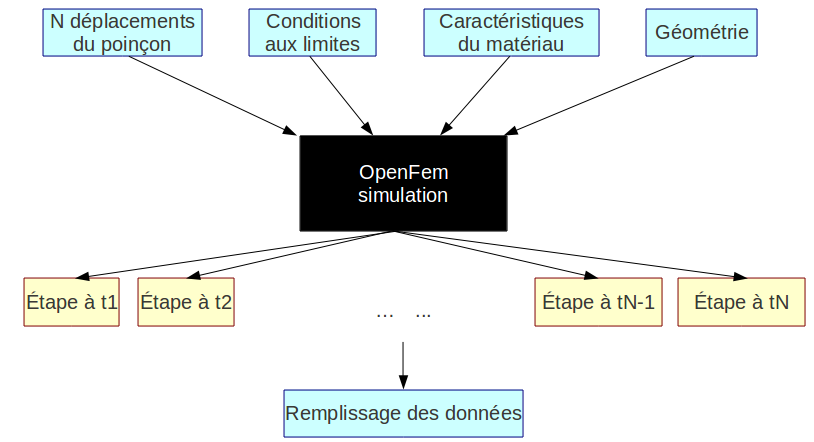
\includegraphics[width=\textwidth]{img/OpenFEM.png}
        \caption{Dialogue avec le moteur de déformation}
    \end{figure}
\end{frame}
\subsection{Liste des livrables}
\begin{frame}
    Concernant la partie Image et CAO:
    \begin{itemize}
        \item Visualisation grâce au lecteur sous forme d'une vidéo ou étape par étape.
        \item Deux intéractions à la souris.
        \item Affichage de l'aire couverte par la tôle.
    \end{itemize}
\end{frame}

\section{Description des méthodes}
\subsection{Méthodologie générale}
\subsection{Méthodes utilisées ou envisagées}
\subsection{Procédés de validation}

\section{Résultats}
\subsection{Expérimentations réalisées}
\subsection{Évaluation des résultats}
\subsection{Critiques et commentaires}

\section{Conclusion}
\subsection{Diagrammes de Gantt}
\subsection{Perspectives}
\subsection{Questions}

\end{document}
